\chapter{Pulling on a carbon nanotube}

\vspace{-1cm} \noindent \textcolor{graytitle}{\textit{{\Large Stretching a carbon nanotube until it breaks}}\vspace{0.5cm} }

\noindent \hspace{-0.45cm}\begin{wrapfigure}{r}{4cm}
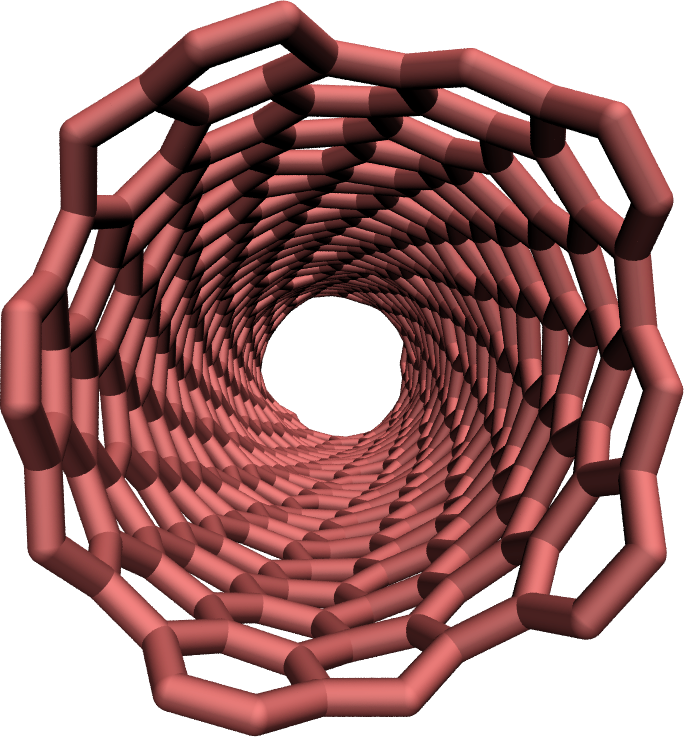
\includegraphics[width=4cm]{tutorials/level1/breaking-a-carbon-nanotube/CNT_light.png}
\end{wrapfigure}

\noindent In this tutorial, a slightly more advanced system than the Lennard-Jones gas
of :ref:`lennard-jones-label` is used.
The system is a small carbon nanotube (CNT) in vacuum, on which some external 
deformation will be applied. Two very different force fields will be used: 
a classical force field, and a reactive force field named AIREBO. With AIREBO,
the breaking of bonds can occur during under strong deformation.

\section{Unbreakable bonds}

\noindent \subsection{System creation}

The initial configuration (atoms positions, bonds, angles,
etc.) is generated using \href{https://www.ks.uiuc.edu/Research/vmd/}{VMD}. Open VMD,
and go to Extensions, Modeling, Nanotube Builder. A window
named Carbon Nanostructures opens up, allowing us to choose
between generating sheet or nanotube of graphene or BN. For
this tutorial, let us generate a carbon nanotube.
Keep all default values, and click on Generate
Nanotube. You should something like the image on the top right 
of this page.
At this point, this is not a molecular dynamics simulation,
but a cloud of unconnected dots. In the VMD terminal, set the
box dimensions by typing the following commands in the VMD terminal:

\begin{lcverbatim}
molinfo top set a 80  
molinfo top set b 80            
molinfo top set c 80 
\end{lcverbatim}

\noindent The values of 80 in each direction have been chosen
so that the box is much larger than the carbon nanotube.
In order to generate the initial LAMMPS data file, let us use Topotool:
to generate the LAMMPS data file, enter the following command:

\begin{lcverbatim}
topo writelammpsdata cnt_molecular.data molecular
\end{lcverbatim}

\noindent Here molecular refers to the LAMMPS \textit{atom$\_$style}, and
\textit{cnt$\_$molecular.data} to the name of the file. 

\begin{tcolorbox}[colback=mylightblue!5!white,colframe=mylightblue!75!black,title=About TopoTools]
Note that I am using TopoTools v1.7. Older or newer versions 
may require slightly different commands. 
More details about these commands can be found on the
personal page of \href{https://sites.google.com/site/akohlmey/software/topotools}{Axel Kohlmeyer}.
In short, Topotools deduces the location of bonds, angles,
dihedrals, and impropers from the positions of the atoms,
and generates a file that can be read by LAMMPS.
\end{tcolorbox}

\noindent The parameters of the constraints (bond length,
dihedral coefficients, etc.) will be given later.
A new file named \textit{cnt$\_$molecular.data} has been created, it starts
like that:

\begin{lcverbatim}
LAMMPS data file. CGCMM style. atom_style molecular generated by VMD/TopoTools v1.7 on Fri Aug 04 11:29:35 CEST 2023
700 atoms
1035 bonds
2040 angles
4030 dihedrals
670 impropers
1 atom types
1 bond types
1 angle types
1 dihedral types
1 improper types
-40.000000 40.000000  xlo xhi
-40.000000 40.000000  ylo yhi
-12.130411 67.869589  zlo zhi

(...)
\end{lcverbatim}

\noindent The \textit{cnt$\_$molecular.data} file contains information
about the positions of the carbons atoms, as well as the
identity of the atoms that are linked by bonds, angles, dihedrals,
and impropers constraints.
Save the \textit{cnt$\_$molecular.data} file in the same folder as your
future LAMMPS input script.
We are done with the system
generation, we can start the molecular dynamics simulations.
Alternatively, you can download the file I did generate 
by clicking  \href{../../../../../inputs/level1/breaking-a-carbon-nanotube/unbreakable-bonds/cnt_molecular.data}{here}, and continue with the tutorial.

\subsection{Generic options}

\noindent Create a new text file and name it \textit{input.lammps}. Copy the
following lines in it:

\begin{lcverbatim}
# Initialisation
variable T equal 300
units real
atom_style molecular
boundary f f f
pair_style lj/cut 14
bond_style harmonic
angle_style harmonic
dihedral_style opls
improper_style harmonic
special_bonds lj 0.0 0.0 0.5
read_data cnt_molecular.data
\end{lcverbatim}

\noindent The chosen unit system is real (distances are in Angstrom, time in femtosecond),
atom style is molecular (atoms are dots that can be bonded with each other),
and the boundary conditions are fixed. The boundary conditions
do not matter much here, as the box boundaries are far from the graphene sheet. 
Here the pair style is lj/cut (i.e. a Lennard Jones potential 
with a short range cutoff) with
parameter 14, which means that the atoms closer than 14
Angstroms from each others interact through a Lennard-Jones
potential. Notice that there is no Coulombic interaction
because there are no partial charges.
The bond, angle, dihedral, and improper styles specify the
different potentials used to restrain the positions of the
atoms. For more details, have a look at the LAMMPS website
(see for example the page of the \href{https://lammps.sandia.gov/doc/dihedral_opls.html}{OPLS dihedral style}).

The last command (\textit{read$\_$data}) imports the carbon.data file
previously generated with VMD, which contains the
information about the box size, atoms positions, etc.

\begin{tcolorbox}[colback=mylightblue!5!white,colframe=mylightblue!75!black,title=About interaction between neighbors atoms]
Atoms connected by a bond do not typically interact through
Lennard-Jones interaction. This is ensured here by the
\textit{special$\_$bonds} command. The three numbers of the
\textit{special$\_$bonds} command are weighting factors for the
Lennard-Jones interaction between atoms connected by bond
(respectively directly bounded $C-C$, separated by two bonds $C-C-C$,
and separated by three bonds $C-C-C-C$). For instance, the
first weighting factor, with a
value of 0, imposes that two atoms connected by a bond do
not interact through a Lennard-Jones potential (therefore
they only interact through the harmonic potential that bond the atoms
of the graphene).
\end{tcolorbox}

\noindent \subsection{Parameters}

We need to specify the parameters of both bonded and
non-bonded functions. Create a new text file in the same
folder and name it \textit{parm.lammps}. Copy the following lines
in it:

\begin{lcverbatim}
pair_coeff 1 1 0.066047 3.4
bond_coeff 1 469 1.4
angle_coeff 1 63 120
dihedral_coeff 1 0 7.25 0 0
improper_coeff 1 5 180
\end{lcverbatim}

\noindent The \textit{pair$\_$coeff} command sets the Lennard-jones parameters
$\epsilon$ and $\sigma$ for the only type of
atom of the simulation: carbon atom of type 1. The
\textit{bond$\_$coeff} provides the equilibrium distance $r_0$ as
well as the spring constant $K$ for the harmonic
potential imposed between two neighboring carbon atoms,
where the potential is $E = K_r ( r - r_0)^2$. The
\textit{angle$\_$coeff} gives the equilibrium angle $theta_0$ and
constant for the potential between three neighbors atoms :
$E = K_\theta ( \theta - \theta_0)^2$. The \textit{dihedral$\_$coeff}
and \textit{improper$\_$coeff} give the potential for the constraints
between 4 atoms. The file PARM.lammps need to be included in the
simulation by adding the following line to input.lammps:

\begin{lcverbatim}
include parm.lammps
\end{lcverbatim}

\noindent \subsection{Prepare initial state}

Depending on VMD and topotool version, the CNT may or may not be centered in 
the box. Let us make sure that we start from a clean initial state by
recentering the CNT at the origin (0, 0, 0). In addition, the box boundaries 
are not symmetric with respect to (0, 0, 0), as seen in \textit{cnt$\_$molecular.data}:

\begin{lcverbatim}
-40.000000 40.000000  xlo xhi
-40.000000 40.000000  ylo yhi
-12.130411 67.869589  zlo zhi

\end{lcverbatim}

\noindent Let us recenter the CNT:

\begin{lcverbatim}
group carbon_atoms type 1
variable carbon_xcm equal -1*xcm(carbon_atoms,x)
variable carbon_ycm equal -1*xcm(carbon_atoms,y)
variable carbon_zcm equal -1*xcm(carbon_atoms,z)
displace_atoms carbon_atoms move ${carbon_xcm} ${carbon_ycm} ${carbon_zcm}
\end{lcverbatim}

\noindent The first command includes all of the atoms of type one
(i.e. all the atoms here) in a group named \textit{carbon$\_$atoms}. 
The 3 variables measure the current position of the group \textit{carbon$\_$atoms}
along all 3 directions, respectively. Then, the displace atoms 
command move the group \textit{carbon$\_$atoms}, ensuring that its center of mass 
is located at the origin (0, 0, 0).
Let us also change the box boundaries:

\begin{lcverbatim}
change_box all x final -40 40 y final -40 40 z final -40 40
\end{lcverbatim}

\noindent \begin{tcolorbox}[colback=mylightblue!5!white,colframe=mylightblue!75!black,title=Note]
Such cleaner and more symmetrical initial state can simplify
future data analysis.
\end{tcolorbox}

\noindent In order to impose a force to the edges of the CNT, let us isolate the
atoms from the two edges of the CNT and place them into different groups.
Later, the displacement will be applied to the atoms of the edges.
Add the following lines to the input script:

\begin{lcverbatim}
variable zmax equal bound(carbon_atoms,zmax)-0.5
variable zmin equal bound(carbon_atoms,zmin)+0.5
region rtop block INF INF INF INF ${zmax} INF
region rbot block INF INF INF INF INF ${zmin}
region rmid block INF INF INF INF ${zmin} ${zmax}
\end{lcverbatim}

\noindent \begin{lcverbatim}
group carbon_top region rtop
group carbon_bot region rbot
group carbon_mid region rmid
\end{lcverbatim}

\noindent The atoms of the edges as selected within the \textit{carbon$\_$top} and \textit{carbon$\_$bot} groups 
are represented with a different color:

\begin{figure}
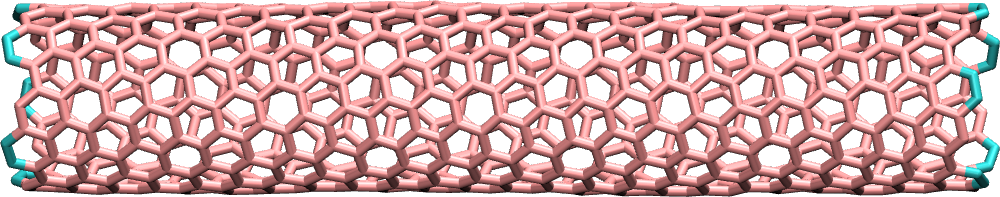
\includegraphics[width=\linewidth]{tutorials/level1/breaking-a-carbon-nanotube/light_colored_edges.png}
\end{figure}

When running a simulation, the number of atoms in each
group is printed in the terminal (and in the log.lammps
file). Always make sure that the number of atoms in each group 
is reasonable, just like here:

\begin{lcverbatim}
10 atoms in group carbon_top
10 atoms in group carbon_bot
680 atoms in group carbon_mid
\end{lcverbatim}

\noindent \subsection{Thermalisation and dynamics}

Let us specify the thermalisation and the dynamics of the
system. Add the following lines to \textit{input.lammps}:

\begin{lcverbatim}
velocity carbon_mid create ${T} 48455 mom yes rot yes
fix mynve all nve
compute Tmid carbon_mid temp
fix myber carbon_mid temp/berendsen ${T} ${T} 100
fix_modify myber temp Tmid
\end{lcverbatim}

\noindent The \textit{velocity$\_$create} command gives initial velocities to
the atoms of the middle group \textit{carbon$\_$mid}, ensuring an initial temperature
of 300 K for these atoms with no overall translational momentum (\textit{mom yes})
nor rotational momentum (\textit{rot yes}).
The \textit{fix nve} is applied to all atoms so that all atom positions are recalculated
every timestep. 

A Berendsen thermostat is applied to the atoms
of the group \textit{carbon$\_$mid} only. The \textit{fix$\_$modify myber} ensures that the
fix Berendsen uses the temperature of the group \textit{carbon$\_$mid} as an
input, instead of the temperature of whole system. This is necessary
to make sure that the frozen edges won't bias the temperature. Note that the atoms
of the edges do not need a thermostat because their motion will
be restrained, see below.

\begin{tcolorbox}[colback=mylightblue!5!white,colframe=mylightblue!75!black,title=Deal with semi-frozen system]
Always be careful when part of a system is frozen. In that 
case, the total temperature of the system is effectively lower
than the applied temperature because the frozen atoms 
have no thermal motion. If you have any doubt about the procedure
you are using, simply check the temperature of the non-frozen group, for
example using the fix ave/time:
\begin{lcverbatim}
fix at1 all ave/time 10 100 1000 c_Tmid file temperature_middle_group.dat
\end{lcverbatim}

\noindent \end{tcolorbox}

\subsection{Deal with frozen edges}

\noindent To restrain the motion of the atoms at the edges, let us add the
following commands:

\begin{lcverbatim}
\end{lcverbatim}

\noindent The two \textit{setforce} commands cancel the forces applied on the
atoms of the two edges, respectively. A fix setforce applies at every step of the
simulation, and are here applying along all 3 directions: $x$, $y$
and $z$. The two velocity commands set the initial velocities along $x$,
$y$, and $z$ to 0 for the atoms of the edges. 

As a consequence of these last four commands, the atoms of the edges will remain
immobile during the simulation (or at least they would if no other command was
applied to them).

\begin{tcolorbox}[colback=mylightblue!5!white,colframe=mylightblue!75!black,title=On imposing a constant velocity to a system]
The \textit{velocity set} commands impose the velocity of a group of atoms when it is 
read, but do not enforce the velocity during the entire simulation. 
When \textit{velocity set} is used in combination with \textit{setforce 0 0 0}, the atoms
wont feel any force during the entire simulation. According to the Newton equation,
no force means no acceleration, meaning that the initial velocity will persist.
\end{tcolorbox}

\noindent \subsection{Data extraction}

Next, in order to measure the strain and stress suffered by the
CNT, let us extract the distance $L$ between
the two edges as well as the force applied on the edges.

\begin{lcverbatim}
variable L equal xcm(carbon_top,z)-xcm(carbon_bot,z)
fix at2 all ave/time 10 100 1000 v_L file length.dat
fix at3 all ave/time 10 100 1000 f_mysf1[3] f_mysf2[3] file force.dat
\end{lcverbatim}

\noindent Let us also add a command to print the atom coordinates in a
lammpstrj file every 1000 steps.

\begin{lcverbatim}
dump mydmp all atom 1000 dump.lammpstrj
\end{lcverbatim}

\noindent \begin{tcolorbox}[colback=mylightblue!5!white,colframe=mylightblue!75!black,title=About extracting quantity from variable compute or fix]
Notice that the values of the force on each edge are
extracted from the fixes setforce \textit{mysf1} and \textit{mysf2}, simply by
calling them using \textit{f$\_$}, the same way variables are called
using \textit{v$\_$} and computes are called using \textit{c$\_$}. A fix
setforce cancels all the forces on a group of atoms at every
step, but allows one to extract the values of the force
before its cancellation.
\end{tcolorbox}

\noindent \subsection{Molecular dynamics run}

Let us run a small equilibration step to bring the system 
to the required temperature without applying any deformation:

\begin{lcverbatim}
thermo 100
thermo_modify temp Tmid
timestep 1.0
run 5000
\end{lcverbatim}

\noindent With the \textit{thermo$\_$modify} command, we specify to LAMMPS that we
want the temperature $T_\mathrm{mid}$ to be printed in
the terminal, not the temperature of the entire system
(because of the frozen edges, the temperature of the entire
system is not relevant). 

\subsection{Option A: Incremental deformation}

\noindent A first possibility to deform the CNT is to 
use the loop function of LAMMPS. 
Let us perform a loop (indentation is optional):

\begin{lcverbatim}
variable var loop 50
\end{lcverbatim}

\noindent At each step of the loop, the edges are slightly displaced, and
the simulation runs for 1000. Then the variable \textit{var} is iterated
by the \textit{next var}, and the simulation \textit{jumps} back to the beginning of 
the loop. It will be repeated 50 times, for a total elongation
equal to $2 \times 0.1 \times 50 = 10$ Angstroms. Increase the number of iteration 
for larger deformation.
You should observe the CNT being progressively elongated
and being deformed.
With the present force field, no matter how large is the
imposed deformation, the bonds will never break. To study
such bond breaking, one has to use a reactive force
field, which is done in some other tutorials here (like :ref:`carbon-nanotube-label`).

\subsection{Option B: Constant-velocity}

\noindent To ensure a smooth step-less deformation of the sheet,
let us impose a constant velocity deformaiton by combining
the \textit{velocity set} command with the \textit{fix setforce}. 
To obtain the same elongation as previously (i.e. 5 Angstrom 
per edge) when using a velocity for each edge of 0.0005 Angstroms per
femtosecond (or 50 meters per second), the simulation 
must last 5 / 0.0005 = 10000 femtoseconds. 
Remove the previous loop and replace it with:

\begin{lcverbatim}
velocity carbon_top set NULL NULL 0.0005
velocity carbon_bot set NULL NULL -0.0005
run 10000
\end{lcverbatim}

\noindent \section{Breakable bonds}

Let us do the same type of simulation, but using a reactive force field 
instead, allowing for the bonds to break.

\subsection{Input file}

\noindent In a different folder, create a LAMMPS input file, call it
input.lammps, and type in it:

\begin{lcverbatim}
# Initialisation
variable T equal 300
units metal
atom_style molecular
boundary p p p
pair_style airebo 2.5 1 1
\end{lcverbatim}

\noindent A difference with the previous part
is the unit system, here \textit{metal} instead of \textit{real}, a choice
that is imposed by the airebo force field.

\begin{tcolorbox}[colback=mylightblue!5!white,colframe=mylightblue!75!black,title=About metal units]
With metal units, the time is in pico second, 
distances are in Angstrom, and the energy is in eV.
\end{tcolorbox}

\noindent Let us prepare the data file. Duplicate the 
previous file \textit{cnt$\_$molecular.data}, name the copy \textit{cnt$\_$atom.data},
place it within the 
current folder, and remove all bond, angle, and dihedral 
information so that \textit{cnt$\_$atom.data} look like that: 

\begin{lcverbatim}
700 atoms
1 atom types
-40.000000 40.000000  xlo xhi
-40.000000 40.000000  ylo yhi
-12.130411 67.869589  zlo zhi
Masses
1 12.010700 # CA
Atoms # molecular
1 1 1 5.162323 0.464617 8.843235 # CA CNT
2 2 1 4.852682 1.821242 9.111212 # CA CNT
(...)
\end{lcverbatim}

\noindent Remove also everything that comes after for \textit{Bonds}
keyword, so that the last lines of the file look like that:

\begin{lcverbatim}
(...)
697 697 1 4.669892 -2.248901 45.824036 # CA CNT
698 698 1 5.099893 -0.925494 46.092010 # CA CNT
699 699 1 5.162323 -0.464617 47.431896 # CA CNT
700 700 1 5.099893 0.925494 47.699871 # CA CNT
\end{lcverbatim}

\noindent The reason the bond information is not needed here is that 
a reactive force field is used. Such force field 
deduces the bonds between atoms on the fly based on the positions of the atoms.
When two initially bonded atoms are separated by a 
distance that is too large, the bond may break. 
You can also download the file I did generate 
by clicking \href{../../../../../inputs/level1/breaking-a-carbon-nanotube/breakable-bonds/cnt_atom.data}{here}.

Then, let us import the LAMMPS data file, and set the
pair coefficients:

\begin{lcverbatim}
# System definition
read_data cnt_atom.data
pair_coeff * * CH.airebo C
\end{lcverbatim}

\noindent Here, there is one single atom type. We impose this type
to be carbon by using the the letter C.
The CH.airebo file can be downloaded \href{../../../../../inputs/level1/breaking-a-carbon-nanotube/breakable-bonds/CH.airebo}{here}.
The rest of the script is very similar to the previous one:

\begin{lcverbatim}
change_box all x final -40 40 y final -40 40 z final -60 60
group carbon_atoms type 1
variable carbon_xcm equal -1*xcm(carbon_atoms,x)
variable carbon_ycm equal -1*xcm(carbon_atoms,y)
variable carbon_zcm equal -1*xcm(carbon_atoms,z)
displace_atoms carbon_atoms move ${carbon_xcm} ${carbon_ycm} ${carbon_zcm}
variable zmax equal bound(carbon_atoms,zmax)-0.5
variable zmin equal bound(carbon_atoms,zmin)+0.5
region rtop block INF INF INF INF ${zmax} INF
region rbot block INF INF INF INF INF ${zmin}
region rmid block INF INF INF INF ${zmin} ${zmax}
group carbon_top region rtop
group carbon_bot region rbot
group carbon_mid region rmid
velocity carbon_mid create ${T} 48455 mom yes rot yes
fix mynve all nve
compute Tmid carbon_mid temp
fix myber carbon_mid temp/berendsen ${T} ${T} 0.1
fix_modify myber temp Tmid
\end{lcverbatim}

\noindent Note that a larger distance was used for the box size along 
the z axis, to allow for larger deformation. The \textit{change$\_$box}
was placed before the \textit{displace$\_$atoms} to avoid issue with the 
CNT crossing the edge of the box.
Let us impose a constant velocity deformation using the atoms
of one edge, while maintaining the other edge fix. Do to so,
one needs to cancel the forces (thus the acceleration) on
the atoms of the edges using the setforce command, and set
the value of the velocity along the z direction.

\subsection{Equilibration}

\noindent First, as an equilibration step, let us set the velocity to 0
for the atoms of the edge. Let us fully constraint the bottom edge, 
and constraint the top edge only along z.

\begin{lcverbatim}
fix mysf1 carbon_bot setforce 0 0 0
fix mysf2 carbon_top setforce NULL NULL 0
velocity carbon_bot set 0 0 0
velocity carbon_top set NULL NULL 0
variable pos equal xcm(carbon_top,z)
fix at1 all ave/time 10 100 1000 v_pos file cnt_deflection.dat
fix at2 all ave/time 10 100 1000 f_mysf1[3] f_mysf2[3] file edge_force.dat
dump mydmp all atom 1000 dump.lammpstrj
thermo 100
thermo_modify temp Tmid
timestep 0.0005
run 5000
\end{lcverbatim}

\noindent At the start of the equilibration, you can see that the
temperature deviates from the target temperature of 300 K, but
after a few picoseconds it reaches the target value:

\begin{lcverbatim}
Step          Temp          E_pair         E_mol          TotEng         Press     
0   300           -5084.7276      0             -5058.3973     -1515.7017    
100   237.49462     -5075.4114      0             -5054.5671     -155.05545    
200   238.86589     -5071.9168      0             -5050.9521     -498.15029    
300   220.04074     -5067.1113      0             -5047.7989     -1514.8516    
400   269.23434     -5069.6565      0             -5046.0264     -174.31158    
500   274.92241     -5068.5989      0             -5044.4696     -381.28758    
600   261.91841     -5065.985       0             -5042.9971     -1507.5577    
700   288.47709     -5067.7301      0             -5042.4111     -312.16669    
800   289.85177     -5066.5482      0             -5041.1086     -259.84893    
900   279.34891     -5065.0216      0             -5040.5038     -1390.8508    
1000   312.27343     -5067.6245      0             -5040.217      -465.74352
(...)
\end{lcverbatim}

\noindent \subsection{Deformation}

After equilibration, let us set the velocity to 30 m/s and run for
a longer time:

\begin{lcverbatim}
# 0.15 A/ps = 30 m/s
velocity carbon_top set NULL NULL 0.15
run 280000
\end{lcverbatim}

\noindent The CNT should break around the step 250000. If not, either 
run for a longer time or for a slightly larger velocity.
When looking at the lammpstrj file using VMD, you will see
the bonds breaking, similar to \href{https://www.youtube.com/watch?v=f1ve1j3yA6w}{this video}. Use
the DynamicBonds representation.

\hspace{-0.45cm}\begin{wrapfigure}{r}{4cm}
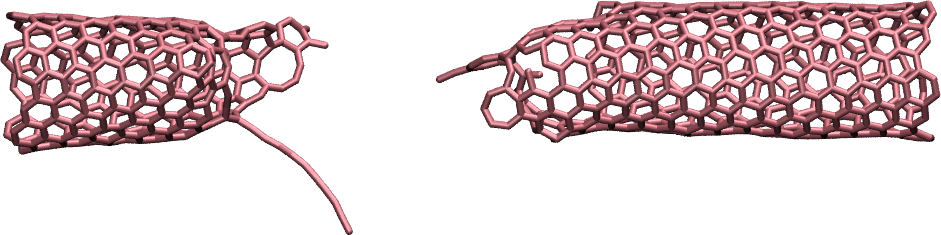
\includegraphics[width=4cm]{tutorials/level1/breaking-a-carbon-nanotube/deformed-light.png}
\end{wrapfigure}

\noindent Figure : Carbon nanotube after being broken.

\begin{tcolorbox}[colback=mylightblue!5!white,colframe=mylightblue!75!black,title=About bonds in VMD]
Note that VMD guesses bonds based on the distances
between atoms, and not based on the presence of actual
bonds between atoms in the LAMMPS simulation. Therefore what is seen
in VMD can sometimes be misleading.
\end{tcolorbox}

\noindent \subsection{Post-mortem analysis (Python)}

There are two main ways to analyse data from a MD simulation:
(1) on-the-fly analysis, like what we did with the two fix ave/time,
and (2) post-mortem analysis. Post-mortem analysis can be performed using
the atom coordinate saved in the lammpstrj file.
Here, let us use the open source Python library MDAnalysis.
Open a new Jupyter notebook within the same folder, call it
\textit{bond$\_$evolution.ipynb}. First, let us import libraries
by copying into \textit{bond$\_$evolution.ipynb}:

\begin{lcverbatim}
import MDAnalysis as mda
import numpy as np
\end{lcverbatim}

\noindent Then, let us create a MDAnalysis universe using the LAMMPS
data file (for the topology information) and the dump file 
(for the coordinate evolution over time). Let us detect the
original bonds using the bond guesser of MDAnalysis. Let us also create 
a single atom group containing all the carbon atoms: 

\begin{lcverbatim}
# create a universe from the dump file
# guess bond based on distance from the initial topology
u = mda.Universe("cnt_atom.data", "dump.lammpstrj",
# create a group
cnt = u.select_atoms("type 1")
\end{lcverbatim}

\noindent Note : The bond guesser of MDAnalysis will not update the list of bond
over time, so we will need to use a few trick.
Then, let us loop over the trajectory and extract bond length and number
over time:

\begin{lcverbatim}
nbond_vs_time = []
lbond_vs_time = []
# loop over trajectory
for ts in u.trajectory:
nbond_vs_time = np.array(nbond_vs_time)
lbond_vs_time = np.array(lbond_vs_time)
\end{lcverbatim}

\noindent The array \textit{nbond$\_$vs$\_$time} contains the number of bond as a function of time, and 
\textit{lbond$\_$vs$\_$time} the bond length. Let us plot both of them:

\begin{figure}
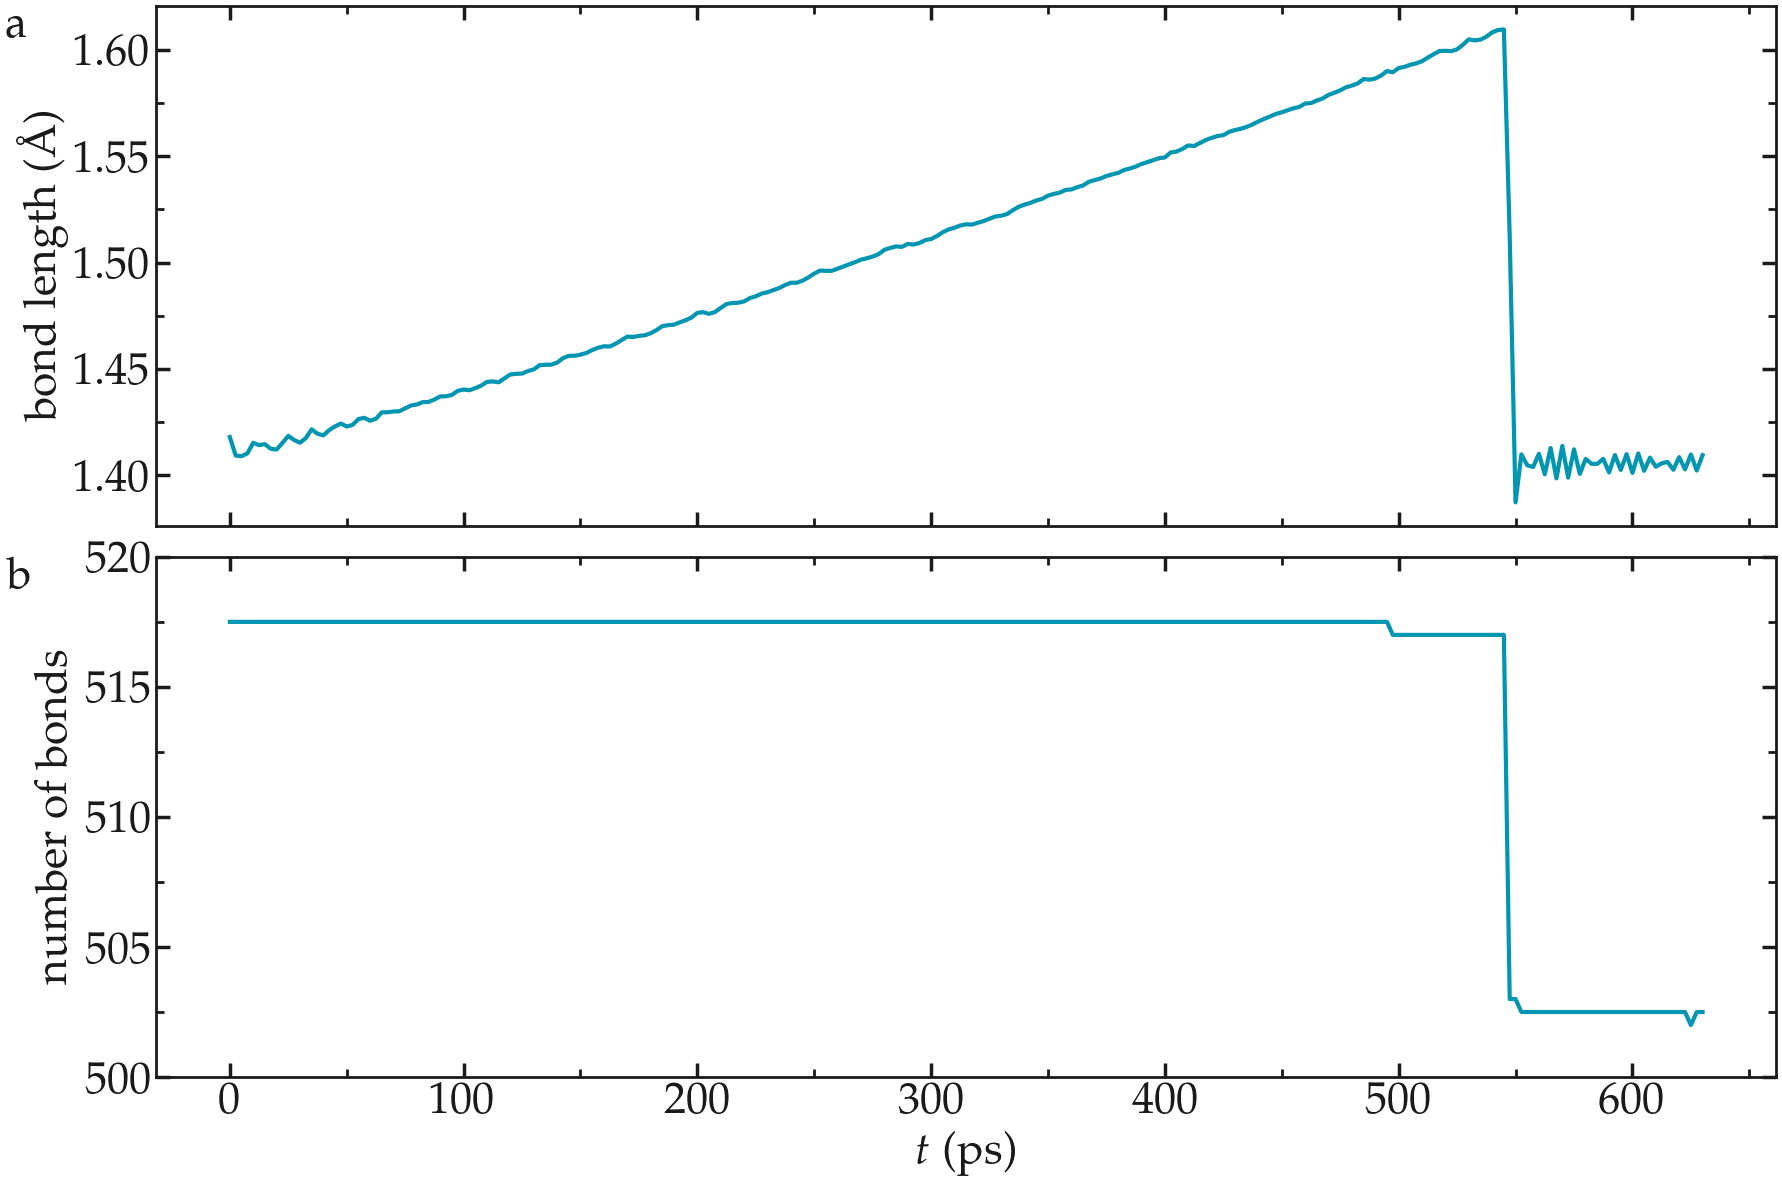
\includegraphics[width=\linewidth]{tutorials/level1/breaking-a-carbon-nanotube/bond-light.png}
\end{figure}

\section{Going further with exercises}

\noindent \subsection{Isolated nanotube}

When a rubber band is streched up, it heats up due to entropy change. 
In the current simulation, the constant exchange of energy with the 
thermostat prevents the temperature to evolve significantly, even under
strong deformation.
Remove the thermostat and observe the evolution of the temperature of an
\textit{isolated} carbon nanotube being deformed. Does it heat-up? Or does it cool down?

\hspace{-0.45cm}\begin{wrapfigure}{r}{4cm}
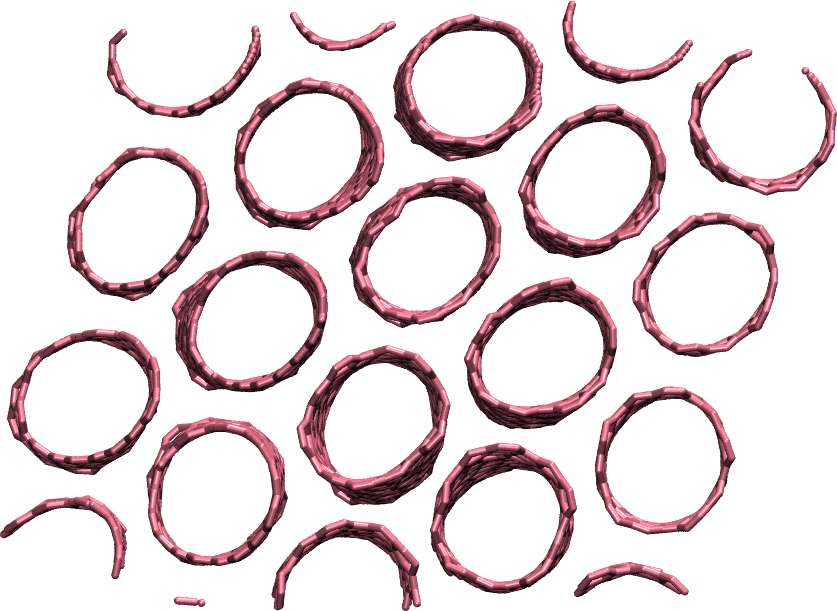
\includegraphics[width=4cm]{tutorials/level1/breaking-a-carbon-nanotube/shared-light.png}
\end{wrapfigure}

\noindent \subsection{Deforming membrane}

Replicate the CNT along x and y, and equilibrate the system to 
create a membrane, just like the image on the right. 
Then, apply a shear deformation along xy.

\begin{tcolorbox}[colback=mylightblue!5!white,colframe=mylightblue!75!black,title=Hints (click to reveal)]
The box must be converted to triclinic to support deformation
along xy.
\end{tcolorbox}

\noindent \hspace{-0.45cm}\begin{wrapfigure}{r}{4cm}
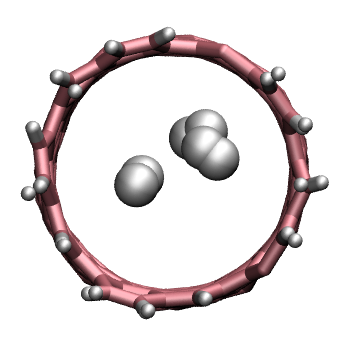
\includegraphics[width=4cm]{tutorials/level1/breaking-a-carbon-nanotube/CH-light.png}
\end{wrapfigure}

\noindent \subsection{Decorate the CNT}

Add hydrogen atoms randomly to the system (using the same
airebo force field). 
Equilibrate the system. After some time, some hydrogen atoms will 
decorate the free carbon atoms at the edge of the CNT. Some 
other hydrogen atoms will bond and form H2 molecules. 

\subsection{Strain-stress curve}

\noindent Adapt the current script and extract a full strain-stress curve.

\begin{figure}
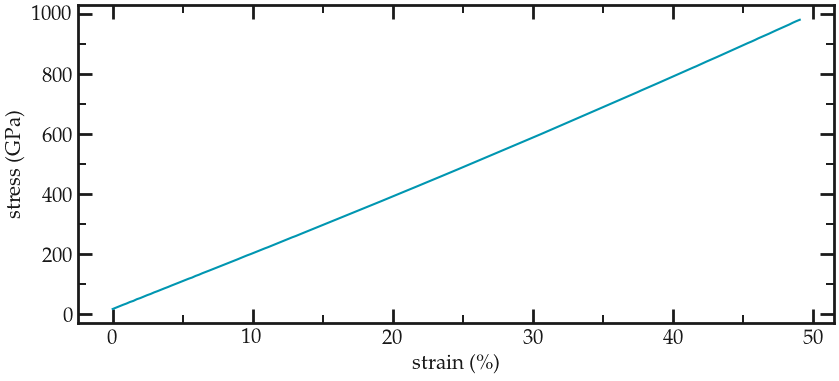
\includegraphics[width=\linewidth]{tutorials/level1/breaking-a-carbon-nanotube/strain-stain-curve-light.png}
\end{figure}

\begin{tcolorbox}[colback=mylightblue!5!white,colframe=mylightblue!75!black,title=Hints]
The following steps are optional, but give a better result:
\begin{itemize}
\item only record data during the production run, not the equilibration
\item reduce the velocity to perform a nice and slow pulling of the graphene sheet
\item increase the magnitude of the total elongation
\end{itemize}
\end{tcolorbox}

